\section{What the design choices do}
\label{sec:controlled}

\begin{figure}[t]
\centering
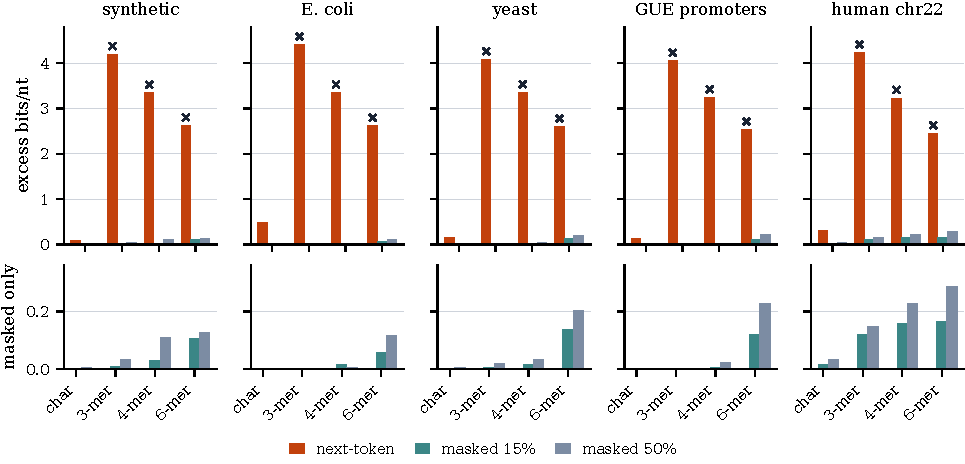
\includegraphics[width=\textwidth]{figures/F1_objective.pdf}
\caption{The objective decides whether records come back; the tokeniser decides how much is stored
either way. One backbone, 30 rounds, canary planted $16\times$, two to three seeds per cell.
\textbf{Top:} \excess{} for the three objectives on all five datasets; a cross marks a cell that
reproduces \emph{every} planted record verbatim. \textbf{Bottom:} the masked cells on their own
scale --- they reproduce nothing anywhere, and within them memorisation still rises with token
length on all five datasets. The masked cells of one dataset also sit within
\NUM{0.05}--\NUM{0.17}\,\bits{} of each other in held-out loss, so the bottom row is already a
matched comparison; the top row is not, which is why the tokeniser axis is read at matched held-out
loss (Table~\ref{tab:controlled-matched}) and never across the top row.}
\label{fig:objaxis}
\end{figure}

\paragraph{The objective decides whether whole records are memorised.}
Decomposing the variance of the $16\times$ canary score over the controlled grid --- one backbone,
four tokenisers, three objectives, two seeds, 24 runs --- attributes \NUM{67.1\%} to the objective,
\NUM{12.0\%} to the tokeniser, \NUM{21.0\%} to their interaction and \NUM{0.0\%} to the seed
(Appendix~A4). The seed term is the reassuring one: at this scale the measurement is
essentially deterministic, so the other three shares are not noise. Once the objective is fixed the
tokeniser is what remains --- \NUM{97.8\%} of the residual variance among the masked cells and
\NUM{100\%} among the next-token cells --- which is the formal version of the two-lever picture in
Fig.~\ref{fig:objaxis}: the objective decides \emph{whether} whole records come back, the tokeniser
decides \emph{how much} is stored either way.

\paragraph{The same decomposition, run before we fixed the placement, says the opposite.}
With every canary copy at the same offset the identical analysis attributes \NUM{59.5\%} to the
tokeniser and \NUM{25.7\%} to the objective: the two leading factors trade places, because a model
with learned absolute positions can score a canary from its position and coarse tokenisers align to
that offset (Appendix~A4). Fixed placement manufactures a tokeniser effect, which is why every
number here uses independently drawn offsets, and the difference between the two decompositions is
larger than most effects anyone would publish from either one.

\paragraph{The tokeniser axis survives the masked objective, two orders of magnitude smaller.}
Under next-token training at a fixed round the four tokenisers sit at held-out losses between
\NUM{2.0} and \NUM{4.4}~\bits, so their \excess{} values are not comparable without the
matched-utility interpolation of Table~\ref{tab:controlled-matched}. Under masked training they
converge on the same budget --- within \NUM{0.05}--\NUM{0.17}~\bits{} inside a dataset --- so that
column is already matched, and in it memorisation is monotone in token length on all five datasets:
the \kmer{6} is the leakiest masked cell everywhere (\NUM{0.12}--\NUM{0.29}) and the character cell
the tightest (\NUM{-0.01}--\NUM{0.03}), with the mask-rate dose--response appearing only where there
is something to dose (\kmer{6}: \NUM{0.12} to \NUM{0.23} between \NUM{15\%} and \NUM{50\%} masking;
nothing resolvable for the character cell).

\begin{table}[t]
\centering
\caption{The tokeniser axis at matched held-out loss, next-token objective, two seeds per cell.
Each entry is verbatim extraction of the $16\times$ canary at the most-overfit end of the loss range
the models share, every model interpolated onto that same held-out loss, so none is read at a
different point of its own trajectory. The \emph{E.~coli} column is a 30-round budget and the other
four are 150 rounds, which is what it takes for the character cell to overfit into a range the
coarse cells also pass through; on human chromosome~22 it never does. The order is monotone in the
average number of nucleotides per token on every dataset, and BPE, whose pieces average 5.0\nt,
lands with the \kmer{6} rather than above both --- the control that separates the tokeniser from the
model, since DNABERT-2 memorises more than any released $k$-mer checkpoint
(Sec.~\ref{sec:published}).}
\label{tab:controlled-matched}
\begin{tabular}{lcccccc}
\toprule
tokeniser & nt/token & synthetic & \emph{E.~coli} & yeast & GUE promoters & human chr22 \\
\midrule
character & 1.0 &   8\% &  0\% &   6\% &   5\% & --- \\
\kmer{3}  & 3.0 &  27\% &  0\% &  40\% &  33\% &  47\% \\
\kmer{4}  & 4.0 &  88\% &  1\% &  93\% &  86\% &  53\% \\
BPE-4096  & 5.0 &  99\% & 28\% & 100\% &  99\% &  86\% \\
\kmer{6}  & 6.0 & 100\% & 53\% & 100\% & 100\% & 100\% \\
\bottomrule
\end{tabular}
\end{table}

\paragraph{Within an objective, memorisation grows with average token length.}
Table~\ref{tab:controlled-matched} reads the $16\times$ canary at matched held-out loss on all five
datasets, and the thresholded statistic separates the cells sharply: at a common held-out loss the
character cell reproduces \NUM{0}--\NUM{8\%} of the planted records, the \kmer{3}
\NUM{0}--\NUM{47\%}, the \kmer{4} \NUM{1}--\NUM{93\%} and the \kmer{6} \NUM{53}--\NUM{100\%}. The
smooth statistic agrees where it can be read: on \emph{E.~coli} \excess{} runs
\NUM{0.32}--\NUM{0.49} for the character cell, \NUM{0.65}--\NUM{0.99} for $k=3,4$ and
\NUM{1.07}--\NUM{1.55} for the \kmer{6} across the shared range.



\begin{figure}[t]
\centering
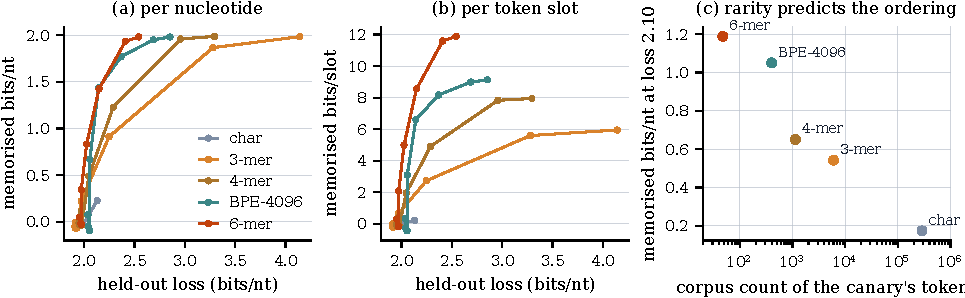
\includegraphics[width=\textwidth]{figures/F2_mechanism.pdf}
\caption{The mechanism, on \emph{E.~coli}, next-token, canary planted $16\times$. (a) and (b) are
the same runs expressed per nucleotide and per token slot: a fixed store per slot would make the
curves collapse in (b), and they spread instead. (c) plots each tokeniser's memorisation at a common
held-out loss against how often the tokens spelling a canary occur elsewhere in the corpus; rarity
orders every cell, including BPE, whose pieces average 5.0\nt.}
\label{fig:mechanism}
\end{figure}

\paragraph{The mechanism is token rarity, not fewer slots.}
A 96\nt{} canary carries the same 192 bits however it is cut; what changes is the number of slots
(96, 32, 24, 16) and how often those tokens occur elsewhere. If a model stored a fixed amount per
slot, the per-nucleotide curves would collapse when re-expressed per slot. They diverge instead,
from a \NUM{7}-fold spread per nucleotide to a \NUM{40}-fold spread per slot
(Fig.~\ref{fig:mechanism}a,b), so slot counting is not the explanation. What does order every cell, on
every dataset we tried, is the corpus count: the tokens spelling a canary occur \NUM{287\,995} times
elsewhere for the character model, \NUM{6014} for the \kmer{3}, \NUM{400} for BPE and \NUM{47} for
the \kmer{6}. A token that almost never occurs elsewhere can be stored without disturbing anything
else the model needs; a frequent one has to be stored together with its context. This also explains
why the effect follows token length rather than vocabulary size: the \kmer{6} and BPE vocabularies
are both about 4100, but their canary tokens differ eight-fold in corpus frequency (Fig.~\ref{fig:mechanism}c).

\paragraph{The same thing happens to sequence we never planted.}
The sharpest objection to a canary study is that inserting a block is itself the effect.
Chromosome~22 repeats sequence on its own, so the objection is testable: we trained the four
tokenisers on 60{,}000 chr22 windows --- above capacity, so the corpus cannot be stored --- and
scored the 96\nt{} blocks the corpus repeats by nature, with nothing planted, against blocks of the
same multiplicity from windows of the same genome the run never trained on, which controls for
repeat families being predictable in themselves (Table~\ref{tab:natural}). A block the corpus
contains \emph{twice} is reproduced verbatim \NUM{63}--\NUM{93\%} of the time when it was trained on
and \NUM{10}--\NUM{23\%} when it was not. So the rulers capture repetition \emph{in training}, not
the predictability of repeats; two copies of real genomic sequence are already enough; and the
tokeniser order holds in this population too (char \NUM{63\%}, \kmer{3} and \kmer{4} \NUM{87\%},
\kmer{6} \NUM{93\%} at multiplicity two). The held-out column carries a result of its own: on
repeats it has never seen, the character model completes \emph{more} than the coarse ones
(\NUM{73\%} against \NUM{43\%} at multiplicity 5--8), so coarse tokenisers memorise more without
generalising better.

\begin{table}[t]
\centering
\caption{Memorisation with nothing planted: verbatim extraction of 96\nt{} blocks that
chromosome~22 repeats by itself, after training on 60{,}000 windows. \emph{Trained} blocks come
from the training set, \emph{held out} blocks of the same multiplicity from windows of the same
genome the run never saw --- the control for repeat families being predictable in themselves.
30 blocks per cell; the full table, including multiplicity $3$--$4$ and $9+$, is in Appendix~A10.}
\label{tab:natural}
\begin{tabular}{lcccccc}
\toprule
& \multicolumn{2}{c}{once} & \multicolumn{2}{c}{twice} & \multicolumn{2}{c}{5--8 times} \\
\cmidrule(lr){2-3}\cmidrule(lr){4-5}\cmidrule(lr){6-7}
tokeniser & trained & held out & trained & held out & trained & held out \\
\midrule
character & 3\%  & 0\% & 63\% & 23\% & 97\%  & 73\% \\
\kmer{3}  & 23\% & 0\% & 87\% & 10\% & 100\% & 60\% \\
\kmer{4}  & 23\% & 3\% & 87\% & 10\% & 97\%  & 57\% \\
\kmer{6}  & 30\% & 0\% & 93\% & 23\% & 100\% & 43\% \\
\bottomrule
\end{tabular}
\end{table}

\paragraph{Neither a small-model artefact nor bought with compute.}
On a 59.9M-parameter backbone (56.7M non-embedding, $4.5\times$ ours, within a factor of two of
DNABERT) both findings reproduce: at matched held-out loss \excess{} runs \NUM{1.06} (character,
\NUM{0\%} extraction), \NUM{2.01} (\kmer{3}, \NUM{5\%}), \NUM{2.04} (\kmer{4}, \NUM{51\%}),
\NUM{2.51} (\kmer{6}, \NUM{100\%}), and every masked cell still reproduces \NUM{0\%} at \excess{}
$\le$ \NUM{0.04}. A character model also processes 288 token slots per window where the \kmer{6}
processes 48, so we re-ran the grid with each cell consuming the same 8.71M supervised tokens
(character 5 rounds, \kmer{3} 15, \kmer{4} 20, \kmer{6} 30). The order is unchanged ---
\NUM{1.32} (\kmer{3}, \NUM{0\%}), \NUM{1.45} (\kmer{4}, \NUM{5\%}), \NUM{1.96} (\kmer{6},
\NUM{76\%}), the character cell never overfitting into the shared range --- and under that budget
the character cell is the \emph{cheapest} in wall clock (14\,s against 35\,s), taking six times
fewer optimiser steps. That last comparison would reverse at longer windows, where attention
dominates.

\paragraph{The length conjecture fails.}
\cite{kharitonov2021bpe} attributed the vocabulary effect in text to the shorter token sequences a
larger vocabulary produces. DNA separates the two: spaced $k$-mer tokenisers hold the token sequence
length fixed while changing the vocabulary, and they reproduce the coarse-tokeniser behaviour, so
length is not the mechanism (Appendix~A3).

\paragraph{What the tokeniser effect is robust to, and what it is sensitive to.}
Every cell has the same 12.61M non-embedding parameters, so only the embedding table changes with
the vocabulary. Three controls rule out the obvious alternatives: factorising the embedding to
rank~512 is a pure reparametrisation yet moves the \kmer{6} to roughly the \kmer{3} level, lowering
only the embedding learning rate makes it memorise \emph{more}, and the character-to-\kmer{3} step
--- parameter-matched to begin with --- is unchanged by both (Appendix~A3). We therefore report the
large-vocabulary excess as a range rather than a constant: for an identical function class it runs
from near zero to large, so memorisation here is a property of the training dynamics and not only of
the architecture. Above capacity the picture sharpens instead: at $20\times$ data the character
model memorises \emph{nothing}, including canaries seen 480 times, while the \kmer{6} recognises
every member canary and extracts every $16\times$ canary verbatim from round~8 (Appendix~A3).
